%!TEX root = ../main.tex

\section{Sensitivity and Regularization}\label{app:activation-pattern-ablations}

This section presents additional ablations studying the sensitivity of the C-ReLU and C-GReLU problems to the selection of the sub-sampled activation patterns, \( \tilde \calD \), and the regularization strength, \( \lambda \).

\textbf{Experimental Details}:
We randomly select 10 datasets from our set of 73 filtered UCI datasets (see \cref{app:uci-datasets}).
For each dataset, we considered thirty individual regularization parameters on log-scale grid over the interval \( [1 \times 10^{-6}, 1] \).
To form the convex formulations, we computed \( \tilde \calD \) by sampling 10, 100, or 1000 generating vectors from \( \calN(0, \bfI) \).
We repeated the sampling procedure with \( 10 \) different random seeds, giving a final total of 60 (30 C-ReLU and 30 C-GReLU) optimization problems for each dataset.
These problems were then solved using R-FISTA and our AL method with the default parameters (see \cref{app:default-parameters}).

\textbf{Additional Results}:
Figures~\ref{fig:hp-gated} and~\ref{fig:hp-relu} present results for the C-GReLU and C-ReLU problems, respectively.
Similar to \cref{fig:reg-plot}, a U-shaped bias-variance trade-off is visible as the regularization strength is increased.
This trend is especially noticeable for the \texttt{monks-3} and \texttt{statlog-heart} datasets.
Variance introduced by sampling \( \tilde \calD \) is only significant for \texttt{heart-va}.

\begin{figure}[htpb]
    \centering
    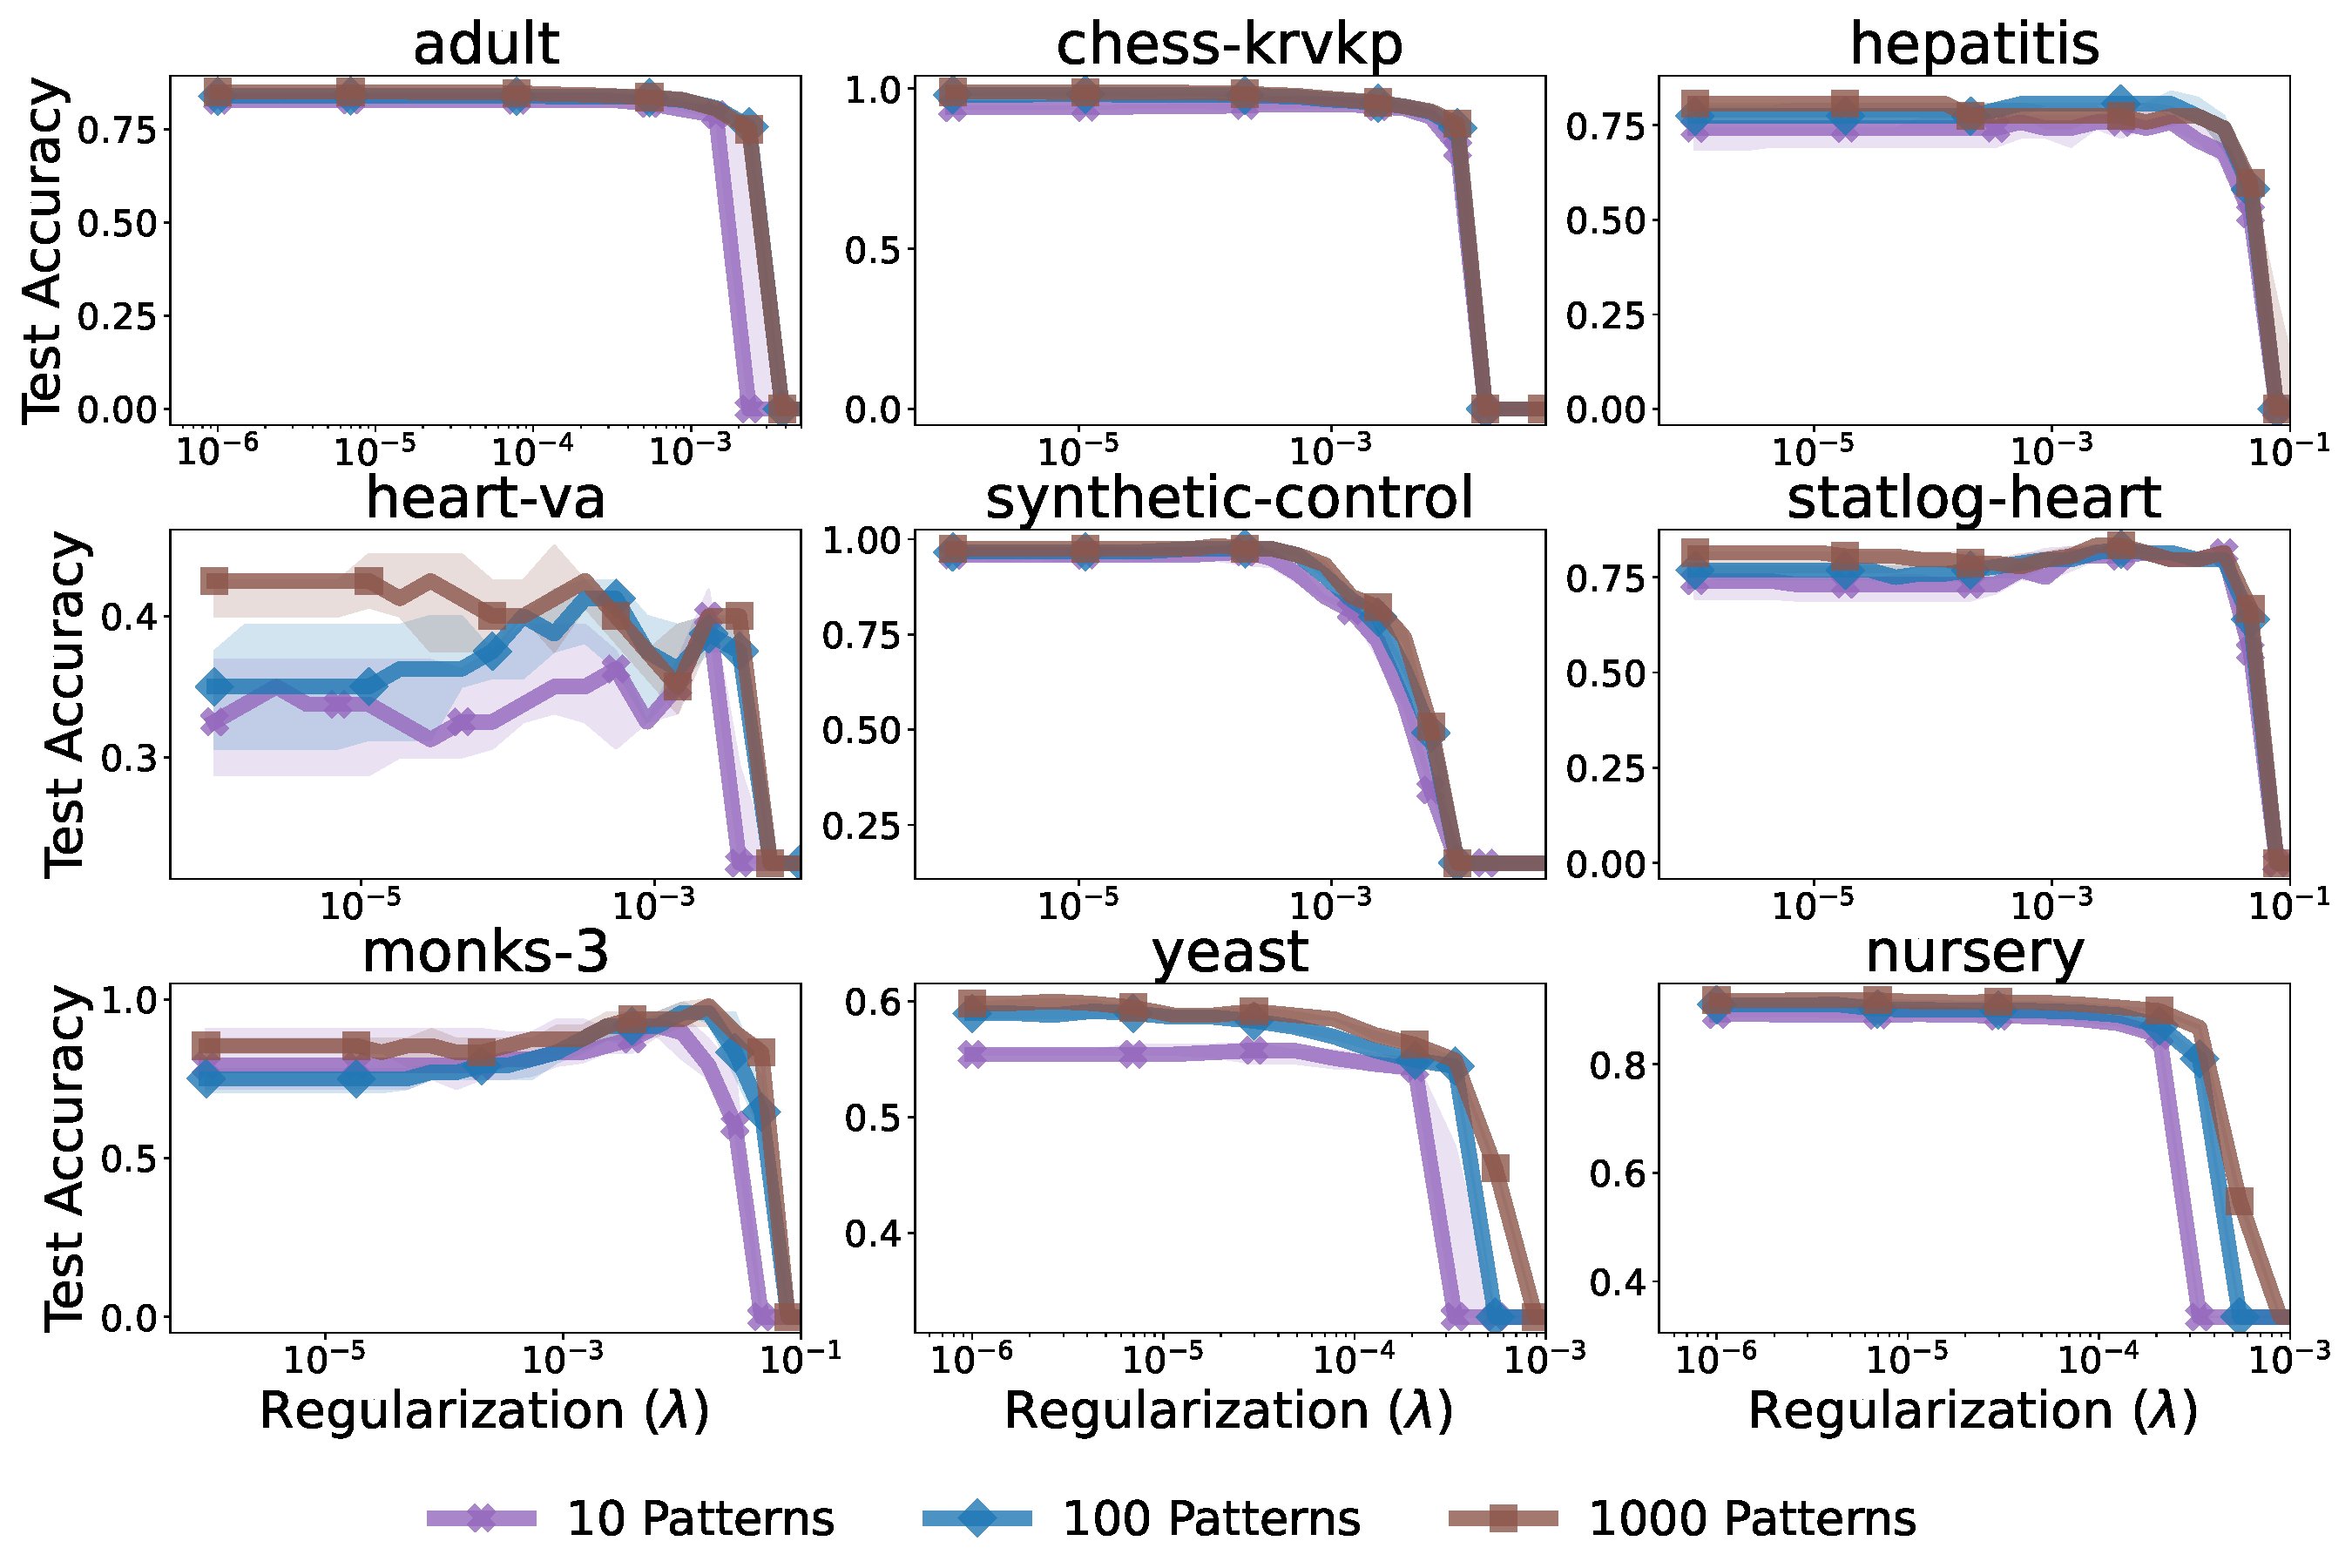
\includegraphics[width=0.85\linewidth]{figures/chapter_two/hp_gated.pdf}
    \caption{
        Effect of sampling activation patterns on test accuracy for neural networks trained using the \textbf{C-GReLU} problem on nine different UCI datasets.
        We consider a grid of regularization parameters and plot median (solid line) and first and third quartiles (shaded region) over 10 random samplings of \( \tilde{\calD} \), where \( |\tilde{\calD}| \) is limited to 10, 100, or 1000 patterns.
    }%
    \label{fig:hp-gated}
\end{figure}

\begin{figure}[htpb]
    \centering
    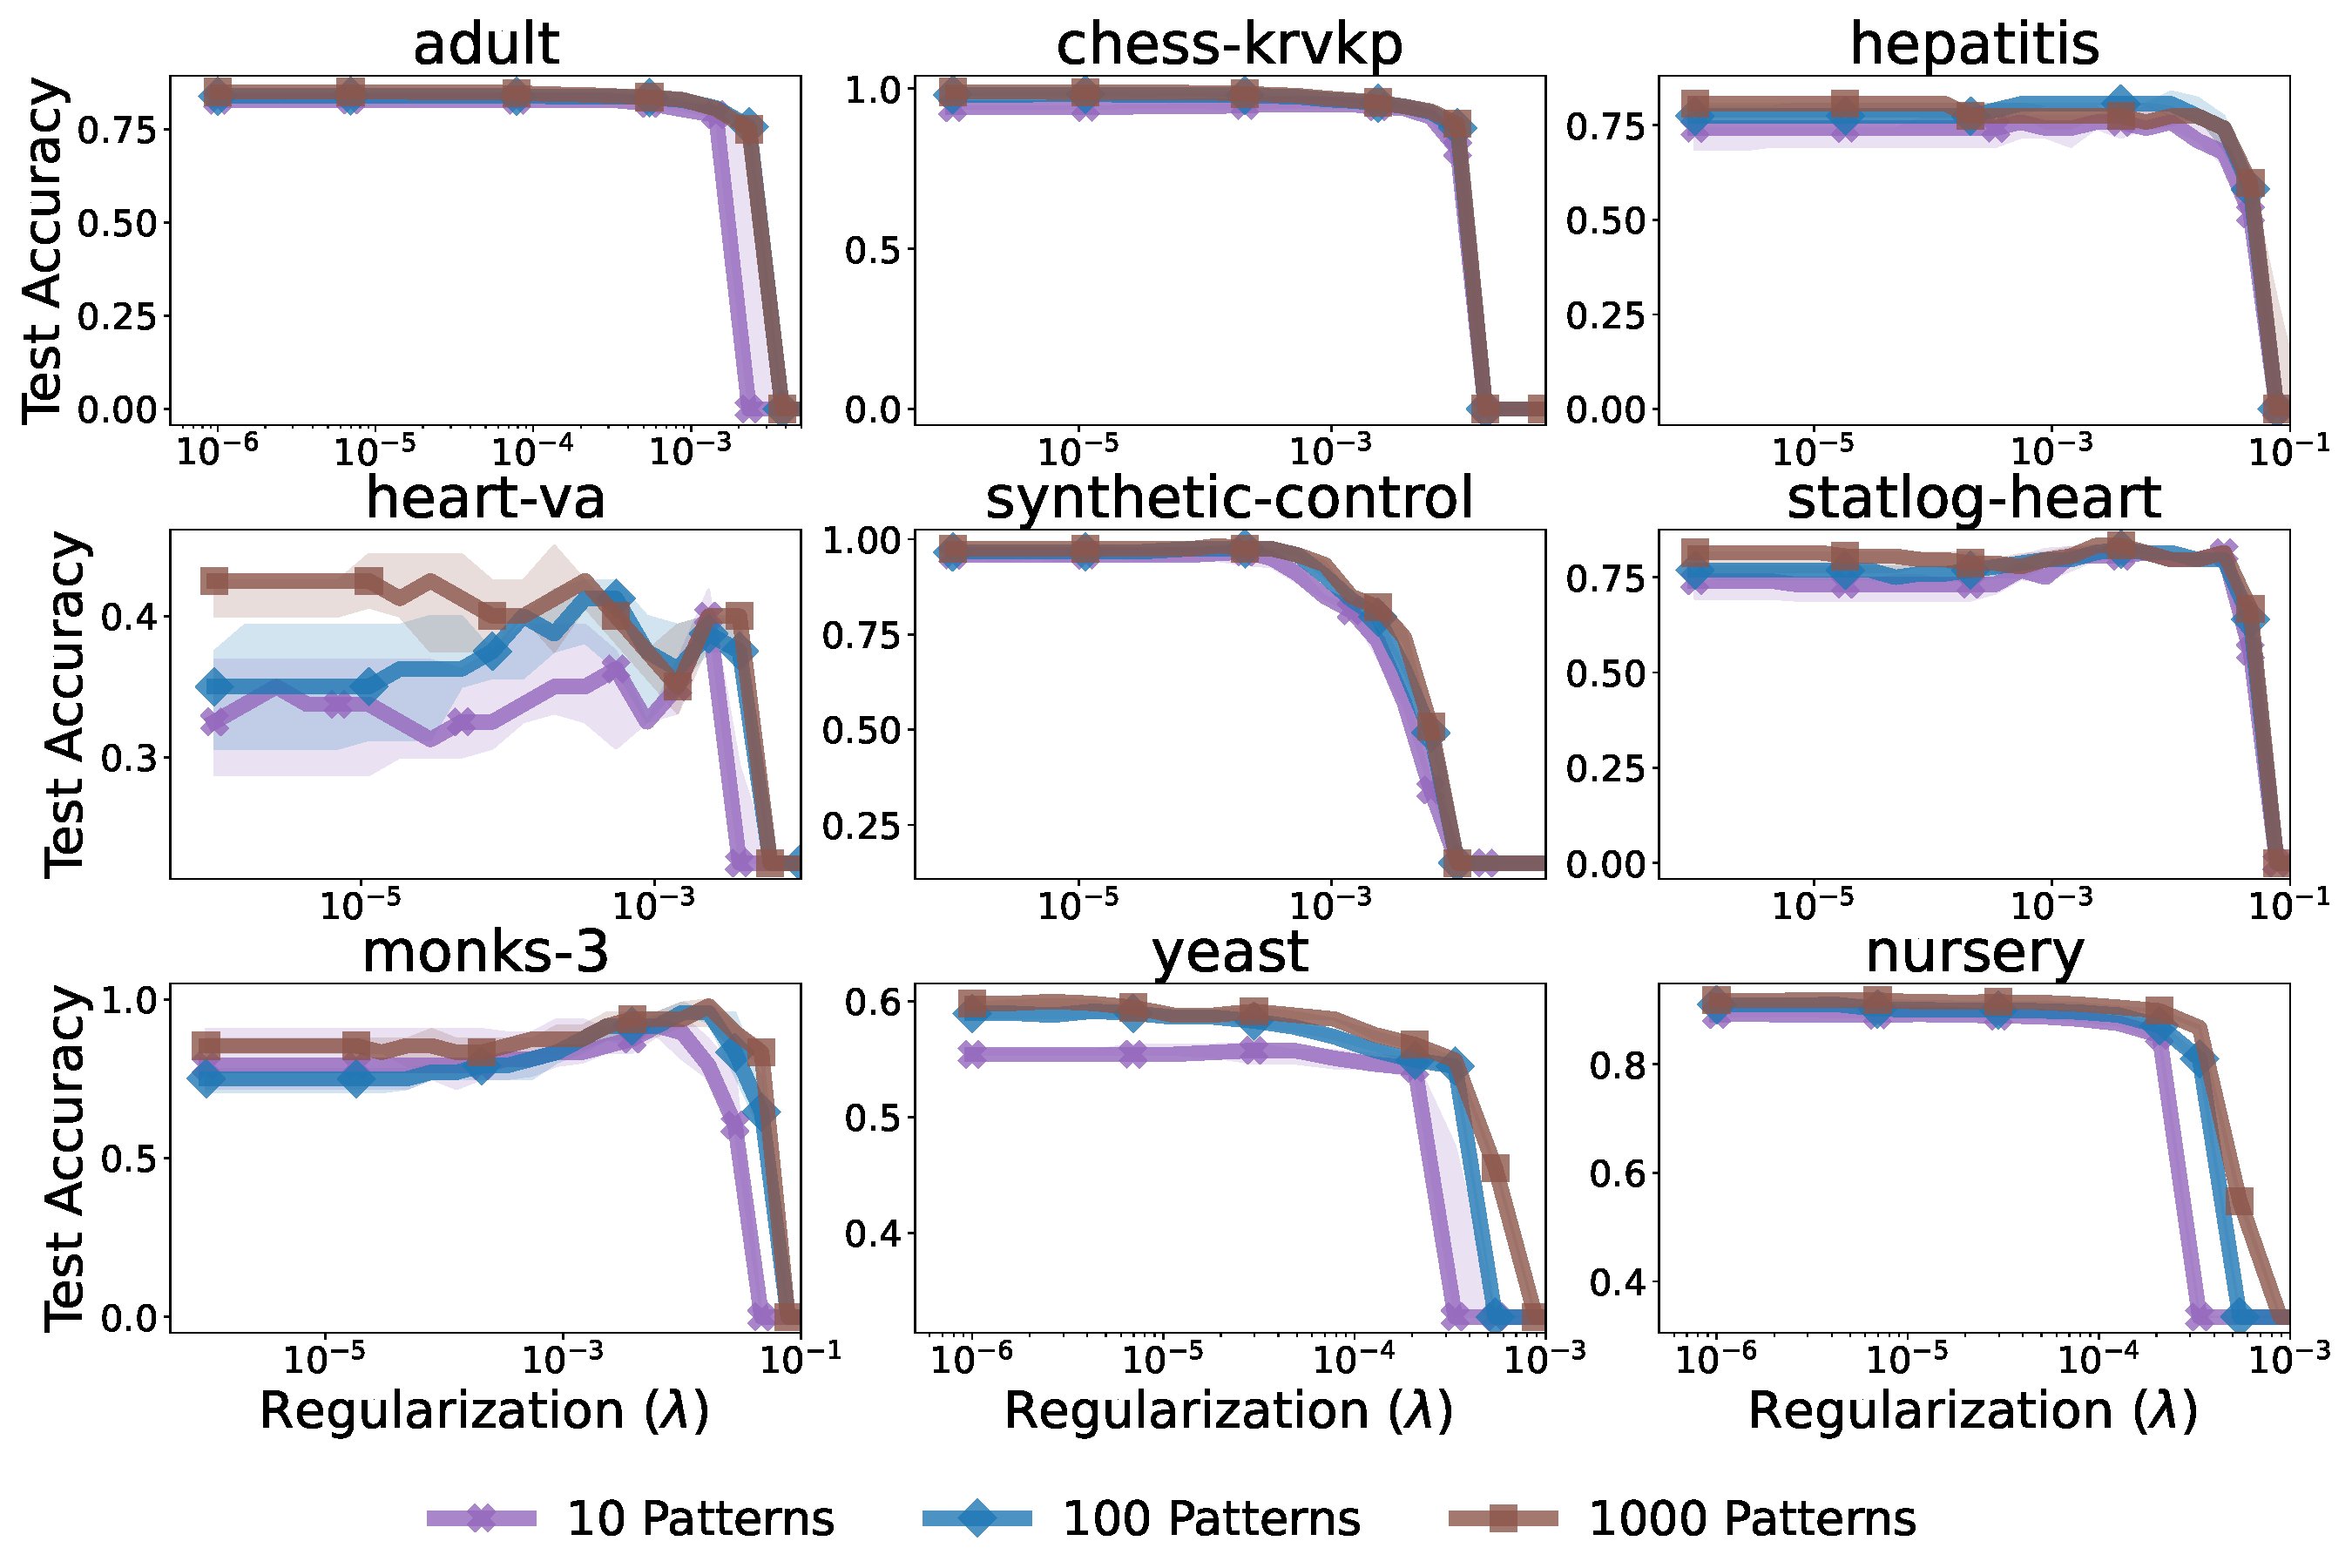
\includegraphics[width=0.85\linewidth]{figures/chapter_two/hp_gated.pdf}
    \caption{
        Effect of sampling activation patterns on test accuracy for neural networks trained using the \textbf{C-ReLU} problem on nine different UCI datasets. See \cref{fig:hp-gated} for details.
    }%
    \label{fig:hp-relu}
\end{figure}
